\chapter{Methodology}

\section{Participants}

For this study, I recruited six Icelandic speakers who were living in York (UK) when the recordings were made.
%TODO Ethic statement
Recruitment was done through University channels, the Icelandic Embassy in London and the York Anglo Scandinavian Society.
All the participants were native speakers of Icelandic, above 18 years old and claimed to have normal hearing and speech abilities.
The information on each participant is given in \Cref{t:participants}.
%TODO Explain table
Participant JR had to be excluded from the analysis since he misunderstood the task, while part of participant SHG's task was lost due to a technical fault in the recording equipment.


\ctable[caption = Information on participants,
label = t:participants,
]{ccccclc}{}{
\FL
id & sex    & age & born & city & languages & abroad \ML
TT & female & 24 & Reykjavik & Reykjavik & English, Danish, German  & Yes \NN
BRS & female & 25 & Hofn      & Hofn      & Danish, English, Spanish & Yes \NN
BTE & female & 27 & Reykjavik & Reykjavik & English, Danish          & Yes \NN
JJ & female & 46 & Reykjavik & Kopavogur & English, Danish          & Yes \NN
SHG & male   & 25 & Selfoss   & Selfoss   & English                  & No  \NN
JR & male   & 66 & Reykjavik & York      & English                  & Yes \LL
}

\section{Materials}

The material used in the task consisted of a list of Icelandic words (the ``target words'') with the following forms: (C)VCC (monosyllabic) and (C)VCCV (bisyllabic).
The list of target words is given in \Cref{a:list}.
The target words were selected so as to control for as many of the following aspects as possible: phonation, manner and place of articulation of consonants following the target vowel; height and frontness of the target vowel; phonation, manner and place of articulation of consonants preceding the target vowel; and height and frontness of the eventual word-final vowel.
Control over these parameters was prioritised according to the order in which they were presented here.
Unfortunately, obtaining a well controlled word list proved to be extremely difficult and several compromises have been made.

%TODO explain words form and how many!


\section{Procedure}

The target words were embedded in the frame sentence \textit{Segðu \_\_ aftur}, `Say \_\_ again.'
This sentence was chosen with the aid of one of the participants so as to control for naturalness, number of syllables and phonetic contexts preceding and following the target word, and phrase stress.
%TODO say why one single frame sentence
The participants were asked to read aloud the sentences with the target words shown on a computer screen.
They were advised to speak as naturally as possible, while keeping the same volume and pace.
They did not familiarised themselves with the word list before starting the task.
The decision of not showing the words beforehand was made to reduce the speakers' control over their speech.
The task was presented through the software PyschoPy \citep{peirce2009}, on a Apple MacBook Pro (mid 2014 model).
Each sentences was shown three times consecutively and the order of appearance was randomised across subjects.
The reading task was self-paced; the participant read a sentence shown on the screen and moved to the next sentence when ready by pressing the space bar.

%TODO add info on recordings
The informants were recorded using a high-fidelity headset microphone plugged into a Zoom H4n Handy Recorder.
The audio files were encoded using the \texttt{.wav} format at a sampling rate of 44 kHz (16-bit).
Four speakers were recorded in a meeting room at a travel agency, while one was recorded at the University of York and the last in his living room, at his house in York.
Even if the recording conditions differed between participants, the quality of the audio is comparable across files.

\section{Measurements}

\begin{figure}
\centering
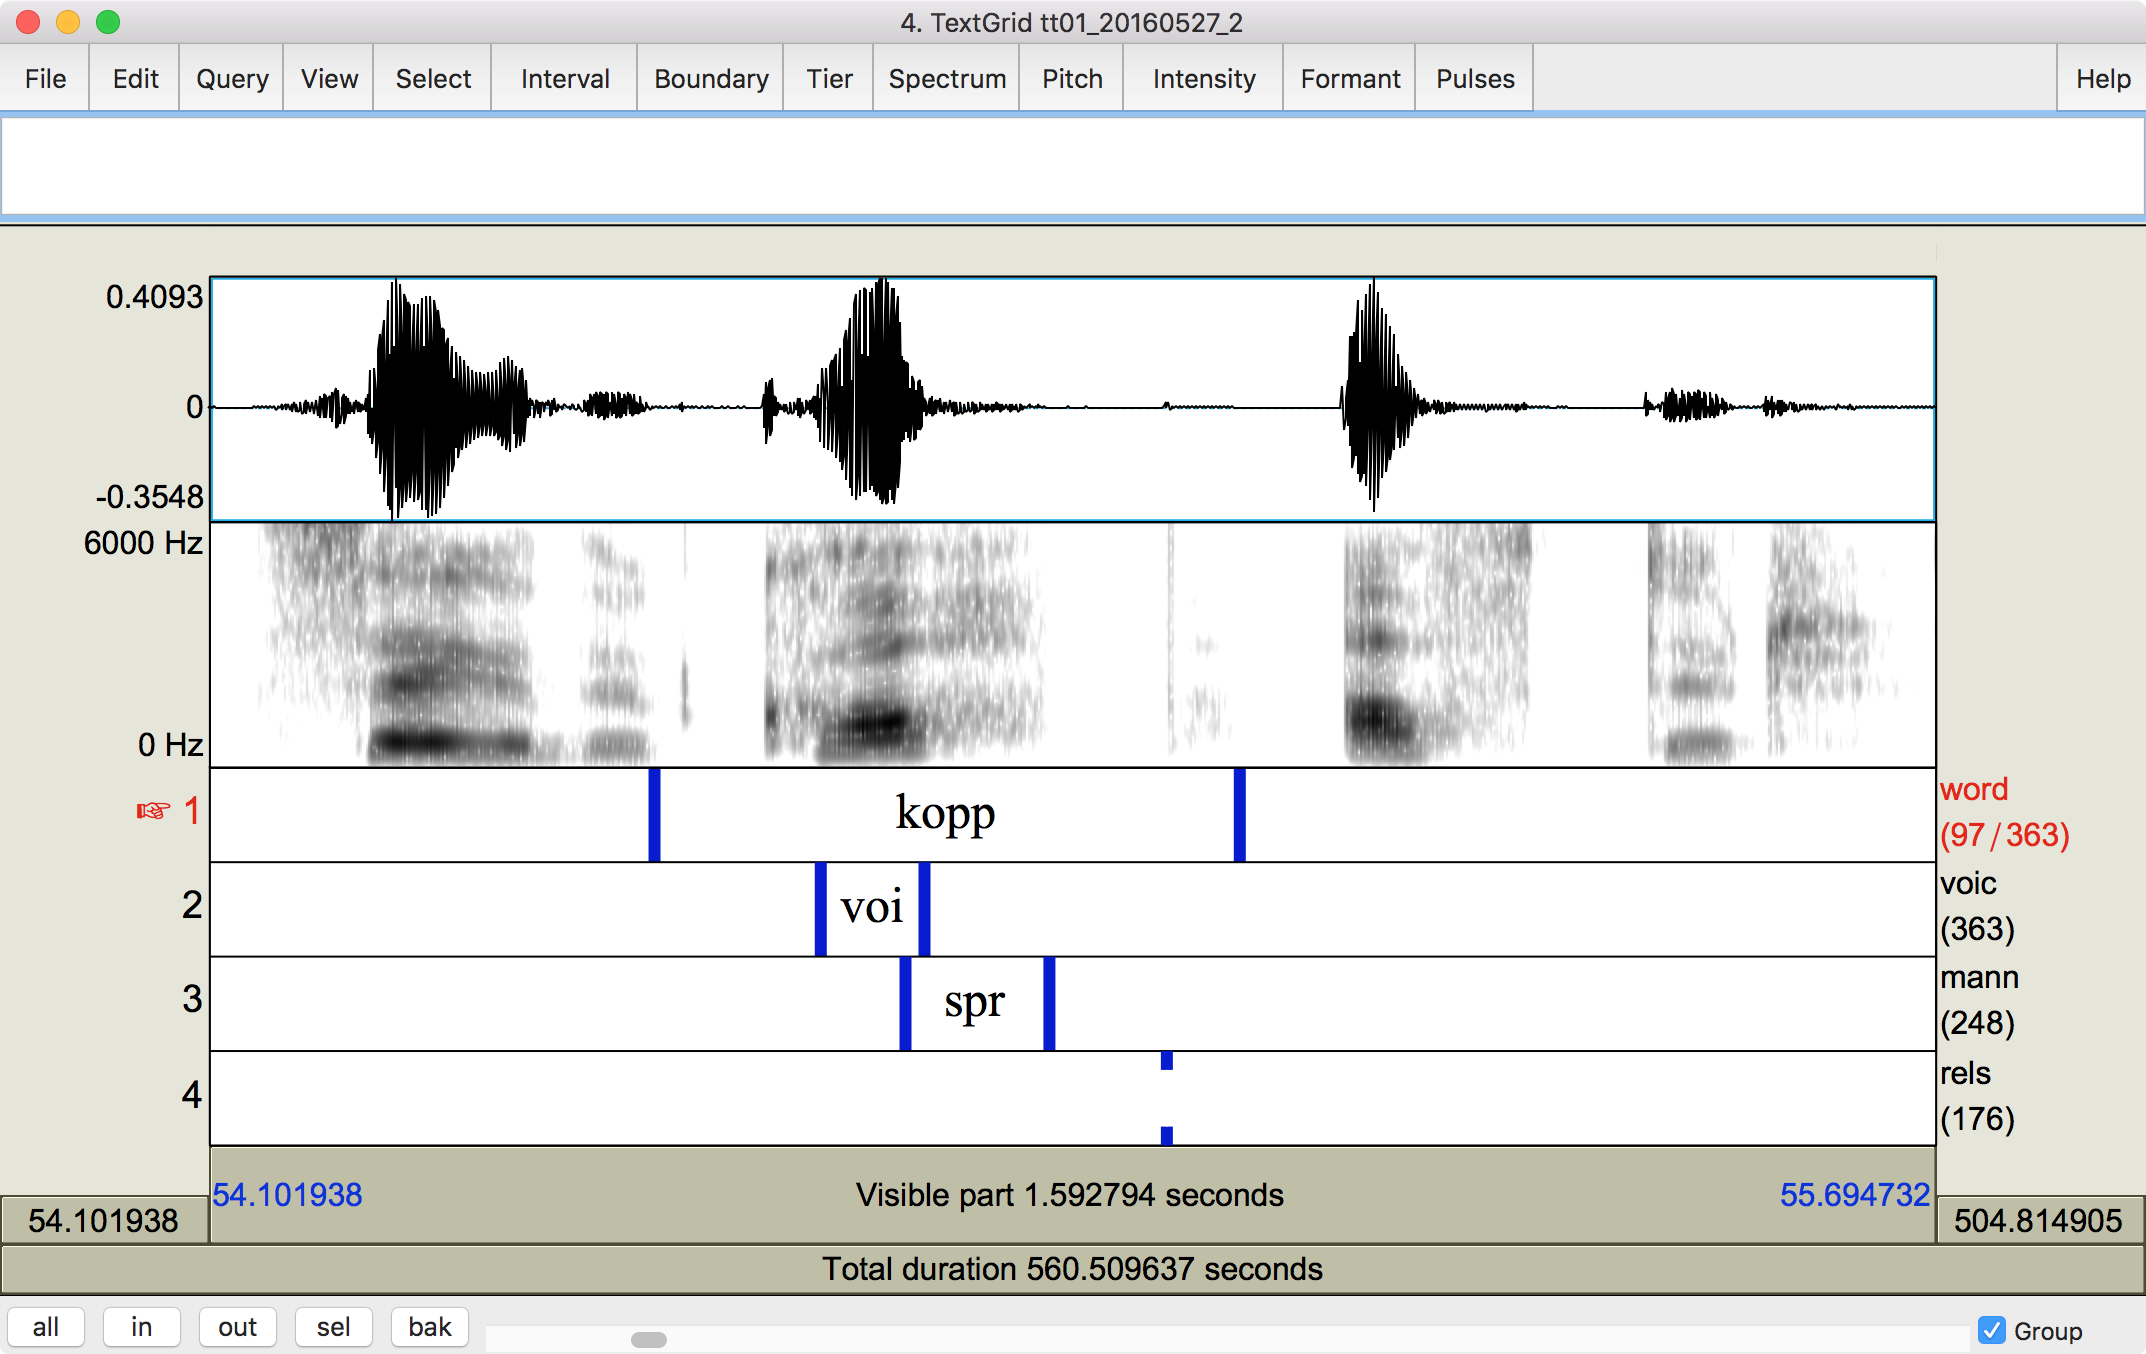
\includegraphics[width=0.7\linewidth]{textgrid}
\caption{TextGrid.}
\label{f:textgrid}
\end{figure}

The analysis of the audio file consisted of three phases:
\begin{inparaenum}[(1)]
	\item conversion from stereo to mono,
	\item annotation, and
	\item extraction of measurements.
\end{inparaenum}
I first converted the audio files from stereo to mono, but I did not apply any filter.
During the second phase, I annotated the files in PRAAT \citep{boersma2015} using TextGrid files.
The annotation files will had four tiers.
The tiers contain, respectively: 
\begin{inparaenum}[(1)]
	\item the graphemic transcriptions of the target words,
	\item the intervals within the words where there is voicing, 
	\item the intervals within the words where laryngeal spread, nasality, laterality or rhoticity is present, and
	\item the release of stops.
\end{inparaenum}
\Cref{f:textgrid} shows an example of the TextGrid set-up.

The first tier was segmented by target words.
The left boundary of the word was considered to be the off-set of voicing of the final vowel of \textit{segðu}, which preceded the target word.
The right boundary differed between consonant-final and vowel-final words.
In consonant-final words, the right boundary coincided with the end of the friction following the burst of the release, as visible in the waveform and spectrogram.
In vowel-final words, the right boundary was placed at the mid-point of the transition between the final vowel and the initial vowel of the following word (\textit{aftur}).
The boundaries of the intervals in the second tier were placed at the on-set and off-set of voicing within the word.
If the word started with one or more voiced continuant consonants, the portion of voicing of those consonants was excluded from the interval and the left boundary was placed at the beginning of the following vowel.

The third tier was used for annotating glottal spread, nasal airflow, laterality and rhoticity.
Marking the beginning of glottal spread proved to be particularly difficult.
%TODO explain how the words were structured prosodically
As in \citet{khan2012}, I expected breathy voice to produce more round-shaped periodic waves.
I took the onset of such more sinusoidal waves to coincide with glottal spread and I marked it as the left boundary of spreading.
The right boundary was assumed to match the end of visible frication noise.
Following standard practice, I marked the beginning of nasality where a change in the shape of the wave and the amplitude in the spectrogram were visible.
I applied the same principle to laterals and rhotics.
I placed the right boundary of these intervals (nasal, lateral, rhotic) depending on the nature of the segment.
The voiceless nasal, lateral and trill consonants terminate with voiceless friction (nareal, lateral or central, respectively).
The end of friction in these consonants was used as the end of the interval.
In the voiced counterparts of these, the end of voicing coincided with the right boundary.
%TODO add pictures
%TODO put what you measured

In the third phase, I extracted the durational properties of the annotated intervals through an automated routine.
The routine was run with a PRAAT script, specifically written for this study.
The script with its documentation can be found in \Cref{a:getmeasure}.
The output is a \texttt{.csv} file with the relevant measurements.
After running the script, I performed the statistical analysis using the R programming language \citep{r-core-team2015} in RStudio \citep{rstudio-team2015}.














